\documentclass[a4paper,12pt,twoside]{article}

\usepackage{../IyA.estilo.2019}
%\usepackage{acronym}	% Inclusi\'on acr\'onimos
			%Definicion acronimo
			%\acrodef{label}[acronym]{written out form}	

%\usepackage[acronym]{glossaries,ifthen,xkeyval,xfor,amsgen}
			%Siempre despues del paquete hyperref

%---------------incorpora acronimos
\newcommand{\acronimo}[1]{\gloss[word]{#1} (\gloss[short]{#1})}
\makegloss


%-------------------para incluir archivos graficos .gif------%
\epstopdfDeclareGraphicsRule{.gif}{png}{.png}{%
  convert gif:#1 png:\OutputFile
}
\AppendGraphicsExtensions{.gif}

\title{S\'intesis de las comunicaciones de a bordo}
\author{Ing. Jorge O. Garc\'ia (jgarcia@efn.uncor.edu)}
\date{\today}

\newcommand{\fullref}[1]{\ref{#1} de la p\'agina \pageref{#1}}

\begin{document}

\renewcommand{\tablename}{Tabla}
\newcommand{\ESPACIO}{\rule{0in}{3ex}}

\maketitle
\thispagestyle{fancy}

\tableofcontents

\newpage

% Capítulo 9. Síntesis de las comunicaciones de a bordo

% 9.1 Comunicaciones en VHF
% 9.2 Comunicaciones en HF



%% Definicion acronimos Sintesis de las comunicaciones de a bordo

			%Definicion acronimo
			%\acrodef{label}[acronym]{written out form}	
%\begin{acronym}[ATC]
  \acrodef{atc}[ATC]{Air Traffic Control}
%\end{acronym}

\section{Introducci\'on}
\label{sec:comunicaciones.a.bordo.introduccion}

Hubo \'epocas en la aviaci\'on en las cuales los pilotos se encontraban volando solos, librados a su suerte, sin posibilidad de comunicarse con otros que se encontraban en tierra o en vuelo.

Con el correr del tiempo se desarrollaron medios de comunicaci\'on utilizando las ondas electromagn\'eticas, con lo cual se logr\'o la transmisi\'on de gran cantidad de informaci\'on a los pilotos, las cuales no consisten s\'olo en comunicaci\'on verbal sino tambi\'en datos necesarios para la seguridad del vuelo.

Hoy en d\'ia resulta dif\'icil imaginar una aeronave, independiente de su tama\~no, sin un sistema de comunicaciones a bordo. A\'un las m\'as peque\~nas pueden contar con un simple transmisor-receptor de radio para sus comunicaciones con tierra, ver Figura \ref{fig:U09.esquema.comunicaciones.actual}.

\begin{figure}[!h]
  \centering
   \includegraphics[width=\textwidth]{Imagenes.U09/comunicaciones.gif}
  \caption{Esquema de comunicaciones actuales}
  \label{fig:U09.esquema.comunicaciones.actual}
\end{figure}

El gran desarrollo tecnol\'ogico de la \'epoca ha hecho posible disponer de equipos de radio aeron\'auticas de diversos tipos, tama\~nos reducidos y gran variedad de posibilidades. 

Los equipos de radios pueden transmitir desde la voz hasta datos y, tambi\'en, modificar de forma aleatoria las frecuencias de emisi\'on (Have Quick), codificando sus transmisiones con claves secretas de forma que s\'olo los equipos que disponen de las mismas puedan comunicarse.


Un equipo de radio a bordo de la aeronave tiene como funci\'on principal comunicarse con los controles de tr\'afico a\'ereo que se encuentran en tierra, \acronimo{ATC}, de forma de proveer un flujo de aeronaves controlado en las operaciones de decolaje y aterrizaje en los aer\'odromos. 

El esquema b\'asico de un sistema de comunicaciones por voz se muestra en la Figura \ref{fig:sistema.radio.x.voz}.

\begin{figure}[!h]
  \centering
  \subfigure[ Emisor de amplitud modulada]{
	\includegraphics[height=6cm]{Imagenes.U09/emisor-am.gif}
	}
  \subfigure[ Receptor de amplitud modulada]{
	\includegraphics[height=6cm]{Imagenes.U09/receptor-am.gif}
	}
  \caption{Sistema de radio por voz}
  \label{fig:sistema.radio.x.voz}
\end{figure}


\section{Espectro de frecuencias}
\label{sec:comunicaciones.a.bordo.espectro.frecuencias}

\gloss{VHF}

\begin{figure}[!htb]
  \centering
 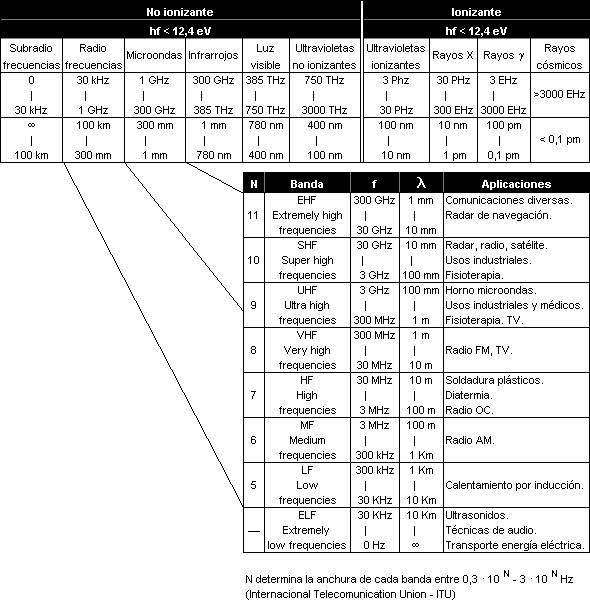
\includegraphics[width=0.9\textwidth]{Imagenes/espectro-frecuencias.jpg} 
  \caption{Espectro de frecuencias, {\tiny Fuente: \url{http://www.siafa.com.ar/notas/nota14/exposicion-radiofrec.htm}}}
  \label{fig:espectro.frecuencias}
\end{figure}


%http://www.siafa.com.ar/notas/nota14/exposicion-radiofrec.htm


\section{Transceptor}
\label{sec:comunicaciones.a.bordo.transceptor}

El transceptor consiste en un equipo combinado de transmisor y receptor que permite emitir se\~nales electromagn\'eticas al exterior de la aeronave y, a su vez, recibirlas.




%\newglossaryentry{VHF}{name=''VHF'',
		description=''Very High Frecuency (Frecuencia muy alta)''
		}

\newacronym{atc}[ATC]{Air Traffic Control}

\newpage
\printgloss{glsbase,tex/comunicaciones-glosario}

%\printglossaries

\newpage

\bibliographystyle{plain}
\bibliography{../IyA}
%\bibliographystyle{plain}
%\bibliography{sample}

\end{document}


%
%  Asi se citan las direcciones web
%
%Example usage
%
%In the preamble:
%---------------
%
%\usepackage{url}
%
%% Define a new 'leo' style for the package that will use a smaller font.
%\makeatletter
%\def\url@leostyle{
%  \@ifundefined{selectfont}{\def\UrlFont{\sf}}{\def\UrlFont{\small\ttfamily}}}
%\makeatother
%
% Now actually use the newly defined style.
%
%\urlstyle{leo}
%
%
%In a BibTeX entry:
%------------------
%
%@misc{
%    c.elmohamed,
%    author = "Saleh Elmohamed",
%    title = "Examples in {H}igh {P}erformance {F}ortran",
%    howpublished = "Website",
%    year = {1996},
%    note = {\url{http://www.npac.syr.edu/projects/
%                    cpsedu/summer98summary/ examples/hpf/hpf.html}}
%}




